\chapter{\IfLanguageName{dutch}{Stand van zaken}{State of the art}}%
\label{ch:stand-van-zaken}

% Tip: Begin elk hoofdstuk met een paragraaf inleiding die beschrijft hoe
% dit hoofdstuk past binnen het geheel van de graduaatsproef. Geef in het
% bijzonder aan wat de link is met het vorige en volgende hoofdstuk.

% Pas na deze inleidende paragraaf komt de eerste sectiehoofding.

In dit hoofdstuk wordt de literatuurstudie besproken over technologieën die essentieel zijn voor het ontwikkelen van een modern e-commerceplatform. De focus ligt op gebruikersauthenticatie met JWT, sessiebeheer via refresh tokens, en de integratie van betalingen via Stripe. Deze componenten vormen de basis van het project.

\section{Gebruikersauthenticatie met JWT}

JWT (JSON Web Token) is een open standaard (RFC 7519) die een compacte en veilige manier biedt om informatie tussen twee partijen uit te wisselen \autocite{Jones2015}. JWT bestaat uit drie delen: een header, een payload en een signature. Deze tokens worden vaak gebruikt voor stateless authenticatie in webapplicaties.

Wanneer een gebruiker succesvol inlogt, genereert de server twee tokens:

\begin{itemize}
\item Een \textbf{access token}, dat een korte levensduur heeft en bij elke API-aanroep wordt meegestuurd in de \texttt{Authorization} header.
\item Een \textbf{refresh token}, dat een langere levensduur heeft en wordt gebruikt om nieuwe access tokens aan te vragen zonder dat de gebruiker opnieuw hoeft in te loggen.
\end{itemize}


In dit project wordt het refresh token \textbf{niet} opgeslagen in een \texttt{HttpOnly} cookie, maar aan de clientzijde (bijvoorbeeld in \texttt{localStorage} of \texttt{sessionStorage}), zoals blijkt uit de configuratie \texttt{api.useSecureCookie=false}. Dit brengt extra aandacht met zich mee voor de beveiliging van de frontend-opslag om risico’s zoals XSS-aanvallen te beperken \autocite{OWASP2021}.

\section{Access- versus Refresh tokens}

Het gebruik van twee soorten tokens biedt een goede balans tussen veiligheid en gebruiksgemak. Access tokens verlopen snel, waardoor ze minder risico vormen bij diefstal. Refresh tokens worden uitsluitend gebruikt om nieuwe access tokens op te halen.

\begin{table}[h]
\centering
\begin{tabular}{l l}
\toprule
\textbf{Token type} & \textbf{Kenmerken} \\
\midrule
Access token & Korte levensduur (bijvoorbeeld 5 minuten), voor API-toegang \\
Refresh token & Lange levensduur (bijvoorbeeld 30 dagen), opgeslagen aan de clientzijde \\
\bottomrule
\end{tabular}
\caption[Verschillen tussen access en refresh tokens.]{Overzicht van de belangrijkste verschillen tussen access- en refresh tokens.}
\end{table}

\section{Betalingen via Stripe}

Stripe is een populaire betalingsprovider met een sterke focus op developer-vriendelijkheid. De Stripe API ondersteunt onder meer betalingen met kredietkaart, Apple Pay en Google Pay \autocite{StripeDocs2024}. In dit project wordt Stripe gebruikt om veilige en betrouwbare betalingen te integreren.

Onderstaand voorbeeld toont hoe een gebruiker hun kaartgegevens kan invoeren en hoe een betaling wordt bevestigd met behulp van de \texttt{stripe.confirmCardPayment}-functie in de frontend.

% \begin{figure}
%   \centering
%   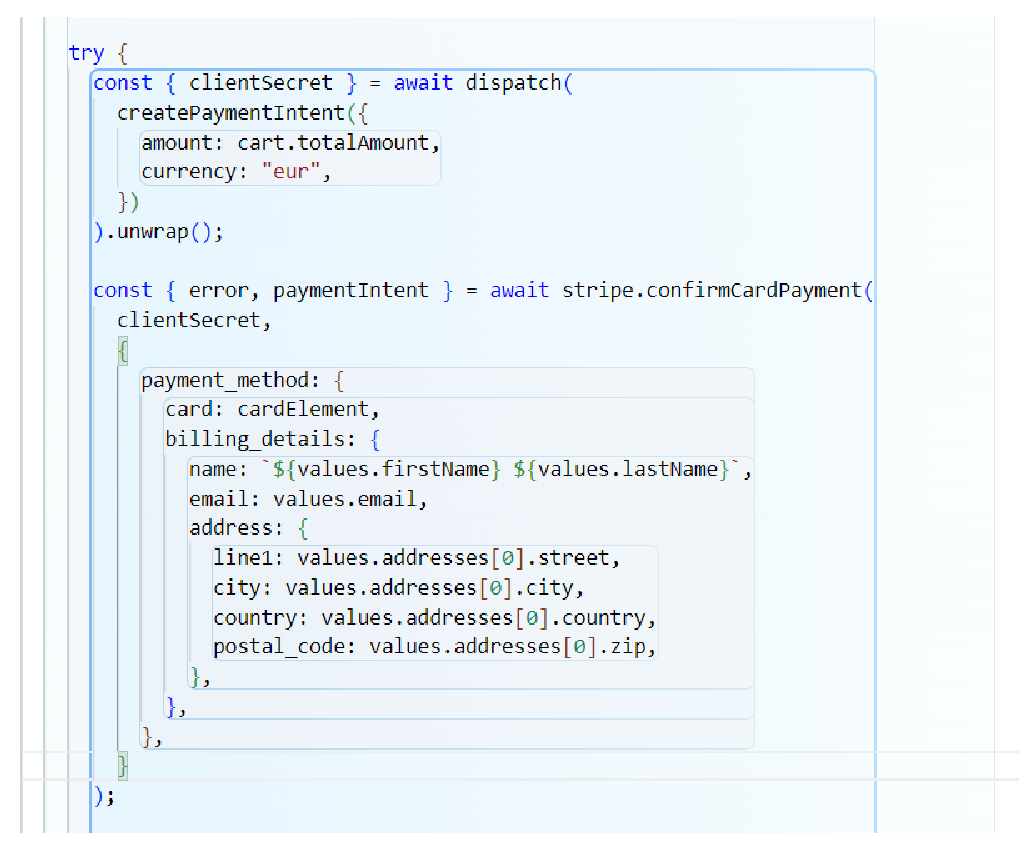
\includegraphics[width=0.8\textwidth]{graphics/codeStripe.eps}
%   \caption[Stripe-integratie in React Checkout-component]{Voorbeeld van een betaling via Stripe in de \texttt{Checkout.jsx} component.}  \caption[Voorbeeld figuur.]{\label{fig:grail}Voorbeeld van invoegen van een figuur. Zorg altijd voor een uitgebreid bijschrift dat de figuur volledig beschrijft zonder in de tekst te moeten gaan zoeken. Vergeet ook je bronvermelding niet!}
% \end{figure}
% \begin{figure}
%   \centering
%   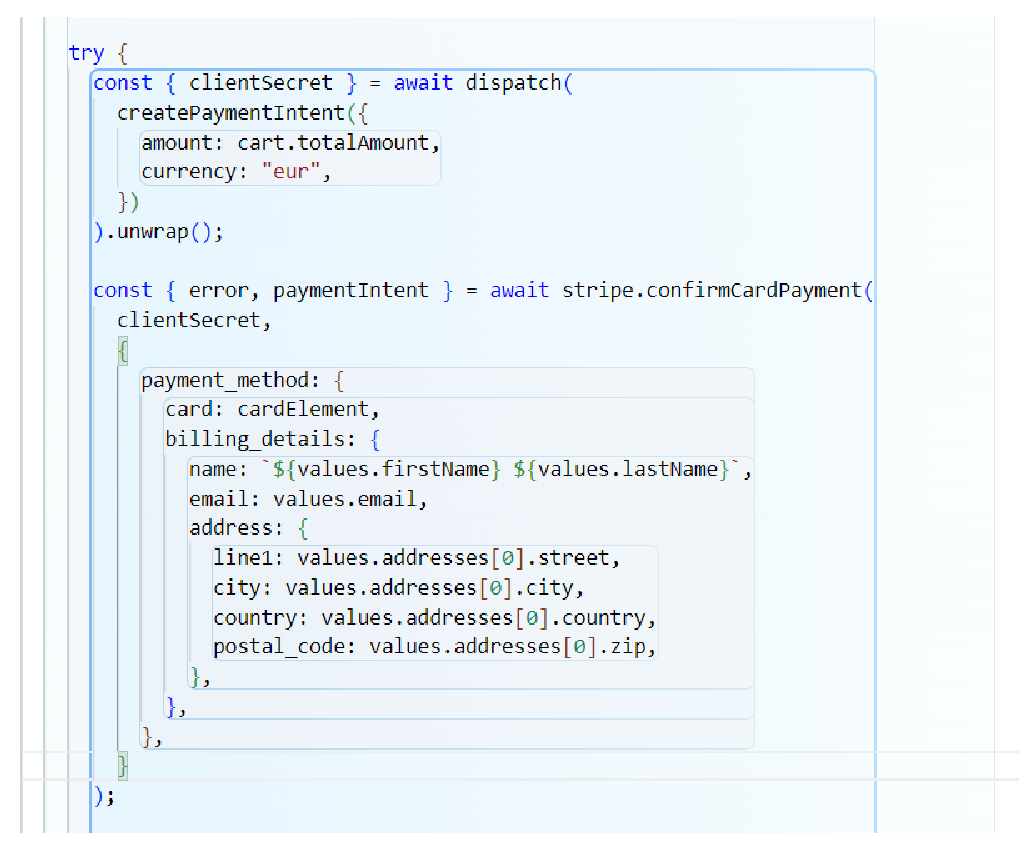
\includegraphics[width=0.8\textwidth]{graphics/codeStripe.eps}
%   \caption[Stripe-integratie in React Checkout-component]{\label{fig:stripe-checkout}Voorbeeld van een betaling via Stripe in de \texttt{Checkout.jsx} component.}
% \end{figure}
\begin{figure}[H]
  \centering
  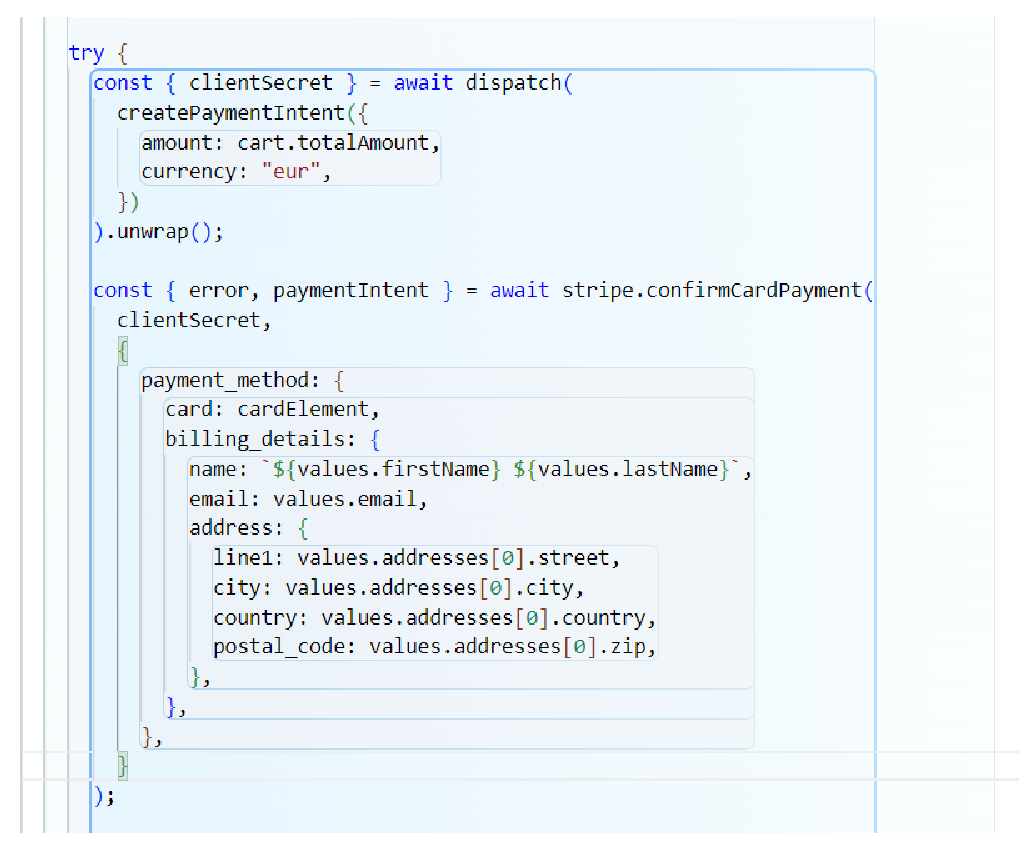
\includegraphics[width=0.8\textwidth]{graphics/codeStripe.eps}
  \caption[Stripe-integratie in React Checkout-component]{\label{fig:stripe-checkout}Voorbeeld van een betaling via Stripe in de \texttt{Checkout.jsx} component.}
\end{figure}

% \label{lst:stripe-checkout}


Het volledige formulier gebruikt \texttt{Formik} en \texttt{Yup} voor validatie en beheert kaartinvoer via de \texttt{CardElement}-component van Stripe. Bij succesvolle betaling wordt de bestelling geplaatst en de winkelwagen gewist.
% \section{Betalingen via Stripe}

% Stripe is een populaire betalingsprovider met een sterke focus op developer-vriendelijkheid. De Stripe API ondersteunt onder meer betalingen met kredietkaart, Apple Pay en Google Pay \autocite{StripeDocs2024}. In dit project wordt Stripe gebruikt om veilige en betrouwbare betalingen te integreren.

% \begin{listing}[h]
% \begin{verbatim}
% Voorbeeld van het starten van een Stripe checkout sessie
% const stripe = await getStripe();
% const { error } = await stripe.redirectToCheckout({ sessionId });
% \end{verbatim}
% \caption[Voorbeeld Stripe-integratie in React]{Codevoorbeeld van Stripe-integratie met React frontend.}
% \end{listing}


\section{Vergelijkbare systemen en best practices}

Platformen zoals Shopify en WooCommerce tonen aan dat een combinatie van JWT-authenticatie, correct beheer van refresh tokens, en betaalintegratie via Stripe een veelgebruikte architectuur is in moderne webshops \autocite{BaeldungJWT,StripeDocs2024}. Best practices benadrukken dat refresh tokens, indien ze niet via \texttt{HttpOnly} cookies worden opgeslagen, op een veilige manier moeten worden beheerd en uitsluitend via beveiligde verbindingen (HTTPS) verzonden moeten worden \autocite{OWASP2021}.